\section{LSTM}
    RNN模型存在的主要问题是,当输入序列过长时,反向传播的计算量过大,实际应用当中大多使用Truncated Backpropagation来处理此问题。
    当然,更好的方法是使用LSTM模型。

    LSTM在RNN的基础上多添加了一个隐藏层cell state,通常用$c_t$来表示,
    此外LSTM还有对应的门控机制来更新模型当中的两个隐藏层,如公式\ref{eq:lstm}所示。
    \begin{equation}
        \begin{aligned}
            \begin{pmatrix}
                i \\ 
                f \\ 
                o \\ 
                g
            \end{pmatrix}
            &=
            \begin{pmatrix}
                \sigma \\ 
                \sigma \\ 
                \sigma \\ 
                \tanh
            \end{pmatrix}
            W
            \begin{pmatrix}
                h_{t-1} \\
                x_t
            \end{pmatrix} \\
            c_t &= f \odot c_{t-1} + i \odot g \\
            h_t &= o \odot \tanh(c_t)
        \end{aligned}
        \label{eq:lstm}
    \end{equation}
    对应的传播模型如图\ref{fig:lstmarchitecture}所示。
    可见,LSTM在反向传播的过程中只需对$c_t$的相关参数进行计算,大幅减少了反向传播的计算量。

    \begin{figure}[H]
        \centering
        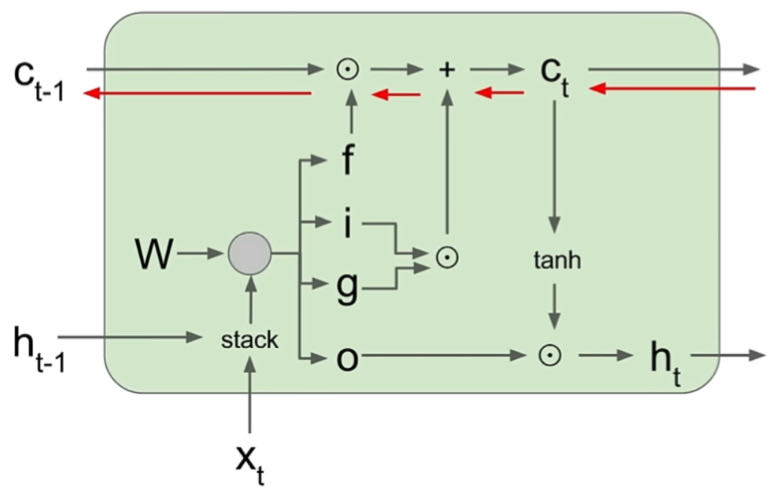
\includegraphics[width=0.4\textheight]{./figures/lstmarchitecture.jpg}
        \caption{LSTM结构}
        \label{fig:lstmarchitecture}
    \end{figure}

    LSTM的训练过程和RNN类似,同样比较有无调度器情况下模型的训练情况,得到的损失曲线如图\ref{fig:lstmlosshistory}所示。
    对应的权重矩阵热力图和文本生成结果参见附录。

    \begin{figure}[H]
        \centering
        \begin{subfigure}{0.45\textwidth}
            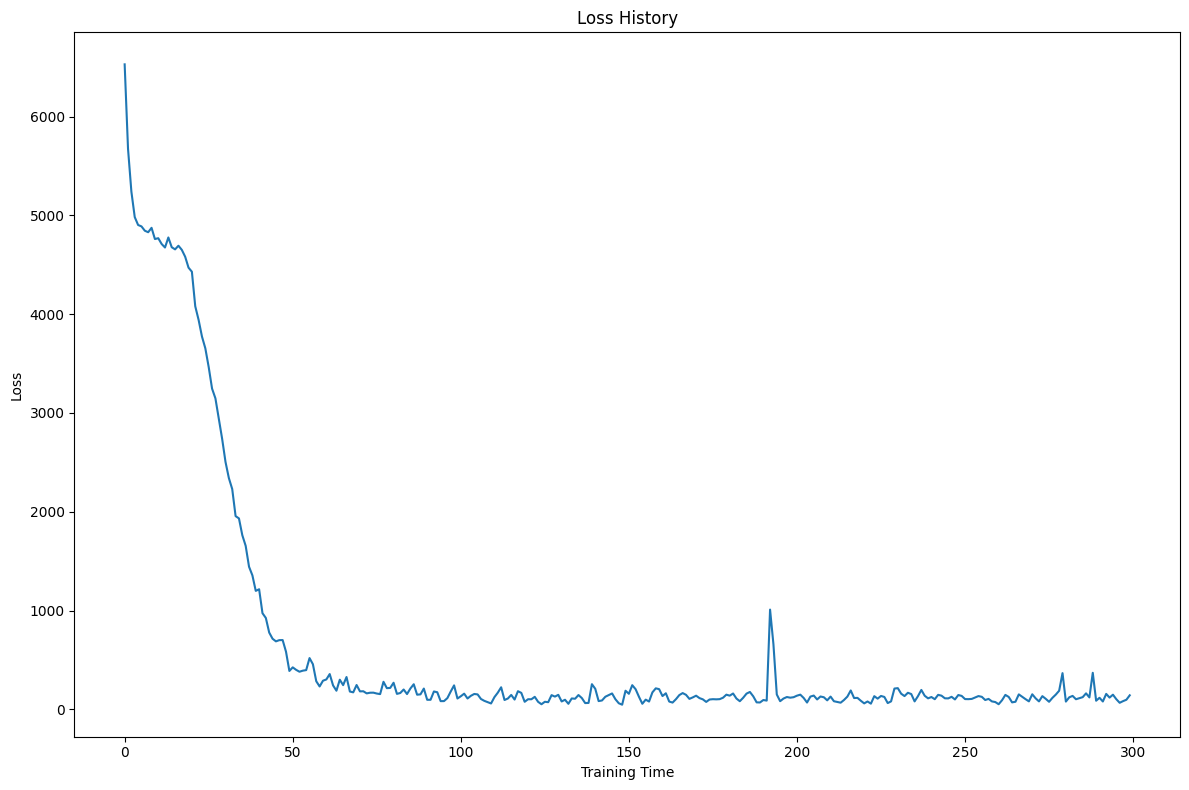
\includegraphics[width=\linewidth]{../output/lstm/no scheduler/lstm_loss.png}
            \caption{不使用调度器}
            \label{fig:LSTMlosshistorynoscheduler}
        \end{subfigure}
        \hfill
        \begin{subfigure}{0.45\textwidth}
            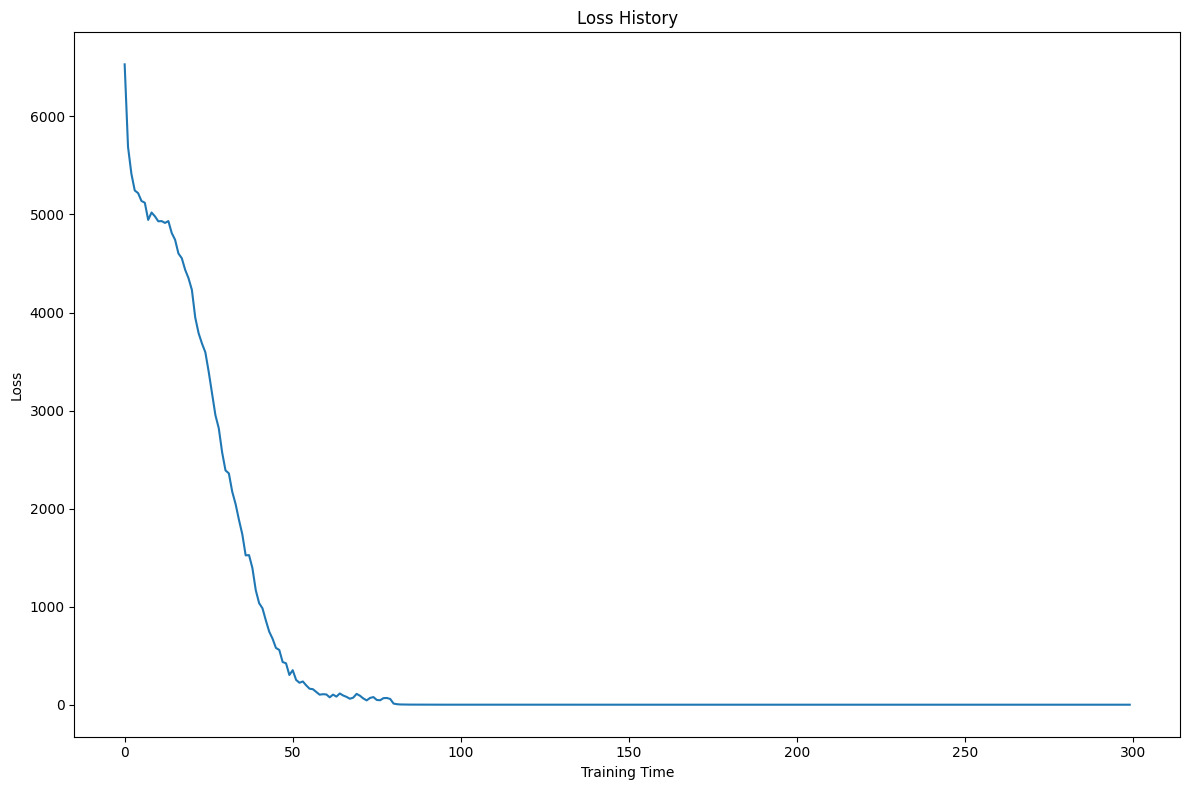
\includegraphics[width=\linewidth]{../output/lstm/with scheduler/lstm_loss.png}
            \caption{使用调度器}
            \label{fig:LSTMlosshistorywithscheduler}
        \end{subfigure}
        \caption{LSTM损失曲线}
        \label{fig:lstmlosshistory}
    \end{figure}

    可以发现,LSTM损失值收敛的速度快于RNN,并且最终收敛的值也远小于RNN的收敛值。
    两者生成的文本中的语法错误数量基本相同。在忽略标点符号以及大小写的情况下,
    不使用调度器时错误数量约为4至6处,使用调度器时错误数量约为2至3处。